\documentclass[letterpaper,10.5pt]{article}
\usepackage[utf8]{inputenc}
\usepackage[T1]{fontenc}
\usepackage[english,spanish,mexico,es-lcroman]{babel}
% Standard packages
\usepackage{float}
\usepackage{ifthen}
\usepackage{xspace}
\usepackage{amsmath}
\usepackage{xstring}
\usepackage{wrapfig}
\usepackage{booktabs}
\usepackage{csquotes}
\usepackage{fancyhdr}
\usepackage{fancyvrb}
\usepackage{geometry}
\usepackage{graphicx}
\usepackage{lastpage}
\usepackage{listings}
\usepackage{multicol}
\usepackage{multirow}
\usepackage{tabularx}
\usepackage{algorithm}
\usepackage{textgreek}
\usepackage[justification=centering]{subcaption}
\usepackage{algpseudocode}
\usepackage[all]{nowidow}
\usepackage[inline]{enumitem}
\usepackage[usenames,dvipsnames]{xcolor}
% Packages to be loaded later
\usepackage{tikz}
\usepackage{cancel}
\usepackage{tcolorbox}
% Include fullpage images with \includepdf
% \usepackage{pdfpages}
% Referencing
\usepackage{varioref}
\usepackage{hyperref}
\usepackage[noabbrev,nameinlink,spanish]{cleveref}
\usepackage[square, comma, numbers, sort&compress]{natbib}


\newcommand{\lpar}{(}\newcommand{\rpar}{)} %CHKTEX 9
\newcommand{\IIC}{I\textsuperscript{2}C\xspace}
\newcommand{\GND}{\textsc{Gnd}\xspace}
\newcommand{\VCC}{\textsc{Vcc}\xspace}
\newcommand{\VDD}{\textsc{Vdd}\xspace}
\newcommand{\textbi}[1]{\textbf{\textit{#1}}}
\newcommand{\degreesC}[1]{%
	#1\textsuperscript{o}C\xspace{}%
}
\newcommand{\degreesF}[1]{%
	#1\textsuperscript{o}F\xspace{}%
}

% \newcommand{\VCC}{V\textsubscript{CC}\xspace{}}
% \newcommand{\GND}{\textsc{Gnd}\xspace{}}
% CHKTEX-FILE 26
% CHKTEX-FILE 36

\tcbuselibrary{most}
% \tcbuselibrary{listings,breakable}
% \usetikzlibrary{shadings,shadows}
% \usetikzlibrary{decorations.pathmorphing}
% \usetikzlibrary{patterns}
% \usetikzlibrary{spy}
% \usetikzlibrary{arrows.meta}

\newtcolorbox{importantbox}[1]{%
	enhanced,
	colback=red!5!white,%
	colframe=red!75!black,%
	fonttitle=\bfseries,%
	center title,
	title={#1},%
	drop fuzzy shadow
}

\newtcolorbox{marker}[1][]{%
	enhanced,
	before skip=2mm,after skip=3mm,
	boxrule=0.4pt,left=5mm,right=2mm,top=1mm,bottom=1mm,
	colback=yellow!50,
	colframe=yellow!20!black,
	sharp corners,rounded corners=southeast,arc is angular,arc=3mm,
%	underlay={%
%		\path[fill=tcbcolback!80!black] ([yshift=3mm]interior.south east)--++(-0.4,-0.1)--++(0.1,-0.2);
%		\path[draw=tcbcolframe,shorten <=-0.05mm,shorten >=-0.05mm] ([yshift=3mm]interior.south east)--++(-0.4,-0.1)--++(0.1,-0.2);
%		\path[fill=yellow!50!black,draw=none] (interior.south west) rectangle node[white]{\Huge\bfseries !} ([xshift=4mm]interior.north west);
%	},
	drop fuzzy shadow,#1
}

%CHKTEX-FILE 1
%CHKTEX-FILE 7
%CHKTEX-FILE 9
% Default fixed font does not support bold face
\DeclareFixedFont{\ttb}{T1}{txtt}{bx}{n}{8} % for bold
\DeclareFixedFont{\ttm}{T1}{txtt}{m}{n}{8}  % for normal

% Custom colors
\usepackage{color}
\definecolor{keywordsColor}{rgb}{0,0,0.5}
\definecolor{customColor}{rgb}{0.6,0,0}
\definecolor{stringColor}{rgb}{0,0.5,0}

% Code highlighting python
\renewcommand{\ttdefault}{pcr}
\lstset{
	language=Python,                              % the language of the code (can be overrided per snippet)
	backgroundcolor=\color{white},                % choose the background color
	basicstyle=\footnotesize\ttfamily,            % the size of the fonts that are used for the code
	breakatwhitespace=false,                      % sets if automatic breaks should only happen at whitespace
	breaklines=true,                              % sets automatic line breaking
	captionpos=t,                                 % sets the caption-position to bottom
	commentstyle=\color{gray},                    % comment style
	deletekeywords={},                            % if you want to delete keywords from the given language
%	escapeinside={\%*}{*)},                       % if you want to add LaTeX within your code
	extendedchars=true,                           % lets you use non-ASCII characters; for 8-bits encodings only, does not work with UTF-8
	frame=tb,                                     % adds a frame around the code
	keepspaces=true,                              % keeps spaces in text, useful for keeping indentation of code (possibly needs columns=flexible)
	keywordstyle=\color{keywordsColor}\bfseries,  % keyword style
	numbers=left,                                 % where to put the line-numbers; possible values are (none, left, right)
	numbersep=5pt,                                % how far the line-numbers are from the code
	numberstyle=\tiny\color{gray},                % the style that is used for the line-numbers
	rulecolor=\color{black},                      % if not set, the frame-color may be changed on line-breaks within not-black text (e.g. comments (green here))
	showspaces=false,                             % show spaces everywhere adding particular underscores; it overrides 'showstringspaces'
	showstringspaces=false,                       % underline spaces within strings only
	showtabs=false,                               % show tabs within strings adding particular underscores
	stepnumber=1,                                 % the step between two line-numbers. If it's 1, each line will be numbered
	stringstyle=\color{stringColor},              % string literal style
	tabsize=2,                                    % sets default tabsize to 2 spaces
	title=\lstname,                               % show the filename of files included with \lstinputlisting; also try caption instead of title
	columns=fixed,                                % Using fixed column width (for e.g. nice alignment)
	otherkeywords={self},                         % if you want to add more keywords to the set
	emphstyle=\color{customColor}\bfseries,       % Custom highlighting style
	emph={__init__,__main__,True,False,None},     % Custom highlighting keywords
	xleftmargin=1cm,                              % Left margin
	xrightmargin=1cm,                             % Right margin
	% Unicode compatibility
	inputencoding=utf8,
	literate={%
	            {Á}{{\'a}}1 {É}{{\'E}}1 {Í}{{\'I}}1 {Ó}{{\'O}}1 {Ú}{{\'U}}1%
	            {á}{{\'a}}1 {é}{{\'e}}1 {í}{{\'i}}1 {ó}{{\'o}}1 {ú}{{\'u}}1%
	            {À}{{\`A}}1 {È}{{\'E}}1 {Ì}{{\`I}}1 {Ò}{{\`O}}1 {Ù}{{\`U}}1%
	            {à}{{\`a}}1 {è}{{\`e}}1 {ì}{{\`i}}1 {ò}{{\`o}}1 {ù}{{\`u}}1%
	            {Ä}{{\"A}}1 {Ë}{{\"E}}1 {Ï}{{\"I}}1 {Ö}{{\"O}}1 {Ü}{{\"U}}1%
	            {ä}{{\"a}}1 {ë}{{\"e}}1 {ï}{{\"i}}1 {ö}{{\"o}}1 {ü}{{\"u}}1%
	            {Â}{{\^A}}1 {Ê}{{\^E}}1 {Î}{{\^I}}1 {Ô}{{\^O}}1 {Û}{{\^U}}1%
	            {â}{{\^a}}1 {ê}{{\^e}}1 {î}{{\^i}}1 {ô}{{\^o}}1 {û}{{\^u}}1% CHKTEX 19
	            {Ã}{{\~a}}1 {Ẽ}{{\~E}}1 {Ĩ}{{\~I}}1 {Õ}{{\~O}}1 {Ũ}{{\~U}}1 {Ñ}{{\~N}}1%
	            {ã}{{\~a}}1 {ẽ}{{\~e}}1 {ĩ}{{\~i}}1 {õ}{{\~o}}1 {ũ}{{\~u}}1 {ñ}{{\~n}}1%
	            {œ}{{\oe}}1 {Œ}{{\OE}}1 {æ}{{\ae}}1 {Æ}{{\AE}}1 {ß}{{\ss}}1%
	            {ç}{{\c c}}1 {Ç}{{\c C}}1 {ø}{{\o}}1 {å}{{\r a}}1 {Å}{{\r A}}1%
	            {€}{{\EUR}}1 {£}{{\pounds}}1 {×}{{\(\times\)}}1% CHKTEX 21
	            {°}{{\textsuperscript{o}}}1%
	            {¹}{{\textsuperscript{1}}}1%
	            {²}{{\textsuperscript{2}}}1%
	            {³}{{\textsuperscript{3}}}1%
	            {⁴}{{\textsuperscript{4}}}1% CHKTEX 19
	            {⁵}{{\textsuperscript{5}}}1% CHKTEX 19
	            {⁶}{{\textsuperscript{6}}}1% CHKTEX 19
	            {⁷}{{\textsuperscript{7}}}1% CHKTEX 19
	            {⁸}{{\textsuperscript{8}}}1% CHKTEX 19
	            {⁹}{{\textsuperscript{9}}}1% CHKTEX 19
	            {⁰}{{\textsuperscript{0}}}1% CHKTEX 19
%	            {A}{{\textAlpha}}1
	            {α}{{\textalpha}}1%
%	            {B}{{\textBeta}}1
	            {β}{{\textbeta}}1%
	            {Γ}{{\textGamma}}1
	            {γ}{{\textgamma}}1%
	            {Δ}{{\textDelta}}1
	            {δ}{{\textdelta}}1% CHKTEX 19
%	            {E}{{\textEpsilon}}1
	            {ϵ}{{\textepsilon}}1%
%	            {Z}{{\textZeta}}1
	            {ζ}{{\textzeta}}1%
%	            {H}{{\textEta}}1
	            {η}{{\texteta}}1%
	            {Θ}{{\textTheta}}1
	            {θ}{{\texttheta}}1%
%	            {I}{{\textIota}}1
	            {ι}{{\textiota}}1%
%	            {K}{{\textKappa}}1
	            {κ}{{\textkappa}}1%
	            {Λ}{{\textLambda}}1
	            {λ}{{\textlambda}}1%
%	            {M}{{\textMu}}1
	            {μ}{{\textmu}}1%
%	            {N}{{\textNu}}1
	            {ν}{{\textnu}}1%
	            {Ξ}{{\textXi}}1
	            {ξ}{{\textxi}}1%
%	            {O}{{\textOmikron}}1
%	            {o}{{\textomikron}}1%
	            {Π}{{\textPi}}1
	            {π}{{\textpi}}1%
%	            {P}{{\textRho}}1
	            {ρ}{{\textrho}}1%
	            {Σ}{{\textSigma}}1
	            {σ}{{\textsigma}}1%
%	            {T}{{\textTau}}1
	            {τ}{{\texttau}}1%
	            {ϒ}{{\textUpsilon}}1
	            {υ}{{\textupsilon}}1%
	            {Φ}{{\textPhi}}1
	            {ϕ}{{\textphi}}1%
%	            {X}{{\textChi}}1
	            {χ}{{\textchi}}1%
	            {Ψ}{{\textPsi}}1
	            {ψ}{{\textpsi}}1%
	            {Ω}{{\textOmega}}1
	            {ω}{{\textomega}}1%
	            {ζ}{{\varsigma}}1%
%	            {}{{\straightphi}}1%
%	            {}{{\scripttheta}}1%
%	            {}{{\straighttheta}}1%
%	            {}{{\straightepsilon}}1%
	         },
}

\lstdefinestyle{c_with_comments}%
{
	language     = c,
	morecomment  = [l]{//},
	morecomment  = [s]{/*}{*/},
	breaklines,
}

\lstdefinestyle{c_without_comments}%
{
	style        = c_with_comments,
	% numbers      = none,
	% keepspaces   = false,
	morecomment  = [l][\nullfont]{//},
	morecomment  = [is]{//}{\^^M},
	morecomment  = [is]{/*}{*/},
}

\lstdefinelanguage{conf}
{
	basicstyle=\ttfamily\small,
	columns=fullflexible,
	morecomment=[s][\color{Orchid}\bfseries]{[}{]},
	morecomment=[l]{\#},
	morecomment=[l]{;},
	commentstyle=\color{gray}\ttfamily,
	% morekeywords={},
	% otherkeywords={=,:},
	% keywordstyle={\color{Green}\bfseries}
}

% \captionsetup[lstlisting]{font={small,tt}}
\captionsetup[lstlisting]{%
	font={small},
}



\DefineVerbatimEnvironment{Verbatim}{Verbatim}{%
	fontsize=\footnotesize,%
	frame=leftline,%
	framesep=2em,    % separation between frame and text
}

\RecustomVerbatimCommand{\VerbatimInput}{VerbatimInput}{%
	fontsize=\footnotesize,
%	frame=lines,            % top and bottom rule only
	frame=leftline,         % left rule only
	numbers=left,           % Line numbers on the left
	numbersep=0.25em,       % Gap between numbers and verbatim lines
	xleftmargin=4em,        % Indentation to add at the start of each line
	xrightmargin=4em,       % Right margin to add after each line
	framesep=0.5em,         % separation between frame and text
	rulecolor=\color{Gray}, % Color of the lines
	labelposition=topline,  %
	samepage=false,         % When true, prevents verbatim environment from
	                        % being broken between pages
%	commandchars=\|\(\),    % escape character and argument delimiters for
	                        % commands within the verbatim
%	commentchar=*           % comment character
}


\hypersetup{
	hidelinks,
	colorlinks=true,
	linkcolor=Blue,
	filecolor=OliveGreen,
	urlcolor=RoyalPurple,
	pdfauthor={Mauricio Matamoros},
%	pdftitle={Práctica 0X – Fundamentos de Sistemas Embebidos},
% 	pdfsubject={The Subject},
% 	pdfkeywords={Some Keywords},
% 	pdfproducer={Latex with hyperref, or other system},
% 	pdfcreator={pdflatex, or other tool}
}

\captionsetup{%
	font=small
}

\geometry{%
	margin=2cm,
	% top=3cm,
	bottom=3cm,
	% left=2cm,
	% right=2cm,
	% inner=2cm,
	% outer=2cm,
	% headheight=,
	% footsep=,
	% footskip=,
}

\pagestyle{fancy}
\renewcommand{\headrulewidth}{0.0pt}
\lhead{}
\chead{}
\rhead{}
\lfoot{}
\cfoot{}
\rfoot{Página~\thepage~de~\pageref{LastPage}}

\crefname{table}{tabla}{tablas}
\Crefname{table}{Tabla}{Tablas}
\crefname{section}{sección}{secciones}
\Crefname{section}{Sección}{Secciones}
\crefname{subsection}{subsección}{subsecciones}
\Crefname{subsection}{Subsección}{Subsecciones}
\crefname{listing}{código de ejemplo}{códigos de ejemplo}
\Crefname{listing}{Código de Ejemplo}{Códigos de Ejemplo}
\renewcommand*{\lstlistingname}{Código ejemplo}


\author{\footnotesize Autor: José Mauricio Matamoros de Maria y Campos}
\title{Práctica 1:\\Instalación de Raspbian en la Raspberry Pi\\
{\large Fundamentos de Sistemas Embebidos}}
\date{}


% Document body
\begin{document}
\maketitle

\section{Objetivo}%
\label{sec:objective}
El alumno aprenderá a instalar un sistema operativo basado en Linux, como sistema operativo embebido, en una tarjeta microcontroladora.

\section{Introducción}%
\label{sec:introduction}
Raspbian es el sistema operativo más popular para Raspberry Pi, además de ser el único con soporte oficial.
Raspbian es una distribución de Linux basada en Debian, optimizado para la Raspberry Pi y que permite a esta operar como una PC.~La distro incorpora terminal y navegador web entre otros programas.

\section{Instrucciones}%
\label{sec:instructions}

Instalar Raspbian en la Raspberry Pi es sencillo.
Basta con descargar Raspbian y grabar la imagen de disco en una tarjeta de memoria microSD, desde la cual arrancará el sistema operativo.

Para esta práctica se necesitará:
\begin{itemize}[nosep]
	\item Una tarjeta de memoria microSD de al menos 4 GB (se recomiendan 8GB)
	\item Una computadora capaz de leer y escribir tarjetas microSD (o bien un adaptador para la misma) y conexión a internet para descargar la imagen de Raspbian.
	\item Una Raspberry Pi 2B o posterior
	\item Un monitor con soporte para HDMI
	\item Un teclado USB
	\item Un mouse USB
	\item Una fuente de alimentación de 5V@1A con adaptador microUSB
\end{itemize}

\paragraph*{Importante:} Si no cuenta con monitor, teclado y mouse, aún es posible instalar Raspbian en la Raspberry Pi. Consulte el \Cref{sec:anex1}.

% %% %%%%%%%%%%%%%%%%%%%%%%%%%%%%%%%%%%%%%%%%%%%%%%%%%%%%%%%%%%%%%%%%%%
%
% Step 1
%
% %% %%%%%%%%%%%%%%%%%%%%%%%%%%%%%%%%%%%%%%%%%%%%%%%%%%%%%%%%%%%%%%%%%%
\subsection{Paso 1: Descargar Raspbian}%
\label{sec:step1}
Ingrese a \url{https://www.raspberrypi.org/downloads/raspbian/} y descargue alguna de las imágenes de Raspbian disponibles (véase \Cref{fig:raspbian-flavors}). Si se descargó un archivo Zip, habrá que descomprimirlo para extraer la imagen.

\begin{figure}
	\centering%
	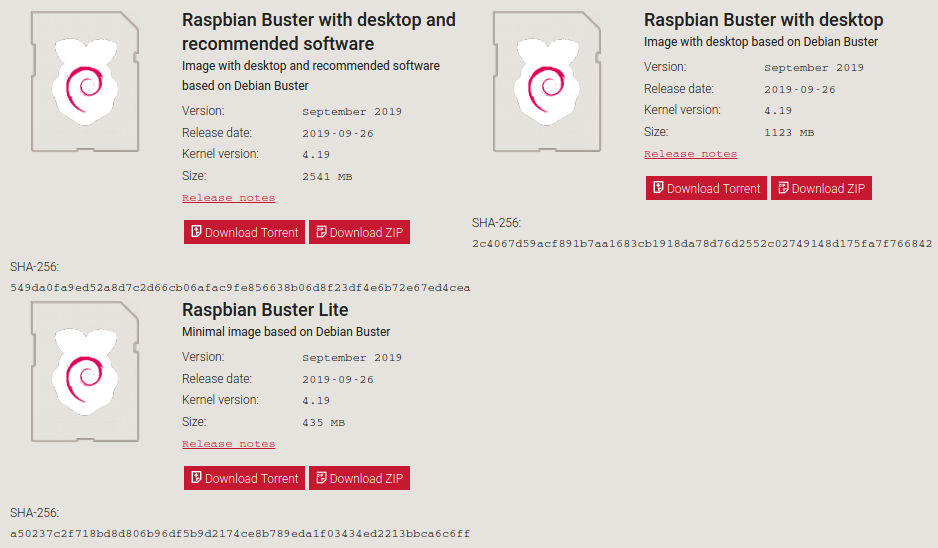
\includegraphics[width=0.8\columnwidth,height=8cm,keepaspectratio]{img/p01-01.png} %CHKTEX 8
	\caption{Versiones disponibles (o sabores) de Raspbian}
	\label{fig:raspbian-flavors} %CHKTEX 24
\end{figure}

La versión a descargar dependerá de la capacidad de la memoria microSD y la cantidad de recursos de la tarjeta Raspbian.
Para tarjetas de 4GB se aconseja el sabor \emph{Raspbian Buster with desktop}, mientras que usuarios con tarjetas de sólo 512MB de RAM querrán instalar \emph{Raspbian Buster Lite}.

Ligas de acceso rápido se proporcionan a continuación por conveniencia:

\begin{itemize}[noitemsep]
	\item \href{https://downloads.raspberrypi.org/raspbian_full_latest}{Raspbian Buster with desktop and recommended software}
	\item \href{https://downloads.raspberrypi.org/raspbian_latest}{Raspbian Buster with desktop}
	\item \href{https://downloads.raspberrypi.org/raspbian_lite_latest}{Raspbian Buster Lite}
\end{itemize}

% %% %%%%%%%%%%%%%%%%%%%%%%%%%%%%%%%%%%%%%%%%%%%%%%%%%%%%%%%%%%%%%%%%%%
%
% Step 2
%
% %% %%%%%%%%%%%%%%%%%%%%%%%%%%%%%%%%%%%%%%%%%%%%%%%%%%%%%%%%%%%%%%%%%%
\subsection{Paso 2: Escribir imagen en la microSD}%
\label{sec:step2}
Si no lo ha hecho, introduzca la memoria microSD en la computadora.
La memoria tendrá que formatearse, por lo que se aconseja respaldar la información.

Escribir la imagen de Raspbian en la microSD requiere de un programa externo según el sistema operativo.

% %% %%%%%%%%%%%%%%%%%%%%%%%%%%%%%%%%%%%%%%%%%%%%%%%%%%%%%%%%%%%%%%%%%%
%
% Step 2a: Linux
%
% %% %%%%%%%%%%%%%%%%%%%%%%%%%%%%%%%%%%%%%%%%%%%%%%%%%%%%%%%%%%%%%%%%%%
\subsubsection{Escribir imagen usando Linux}%
Descargue \href{https://etcher.io/}{Etcher} en \texttt{\textasciitilde/Downloads}, descomprima y ejecute; por ejemplo

\begin{Verbatim}[fontsize=\footnotesize]
$ cd ~/Downloads
$ unzip balena-etcher-electron-1.5.75-linux-x64.zip
$ ./balenaEtcher-1.5.75-x64.AppImage
\end{Verbatim}


A continuación, siga los pasos de Etcher para grabar la imagen (véase \Cref{fig:write-image-linux})
\begin{enumerate}[noitemsep]
	\item Seleccione la imagen IMG de Raspbian
	\item Seleccione el medio en el cual se grabará la imagen de Raspbian (punto de montaje de la microSD)
	\item De click en \emph{Flash!} para empezar el proceso de grabado
\end{enumerate}

\begin{figure}[H]
	\centering%
	\begin{subfigure}[b]{0.5\linewidth}
		\centering
		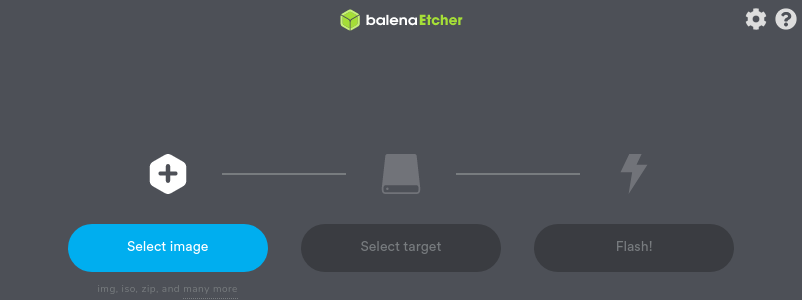
\includegraphics[width=0.9\linewidth,height=8cm,keepaspectratio]{img/p01-02-linux-imagea.png} %CHKTEX 8
		\caption{Selección de imagen a grabar}
		\label{fig:write-image-linux-a} %CHKTEX 24
	\end{subfigure}%
	\begin{subfigure}[b]{0.5\linewidth}
		\centering
		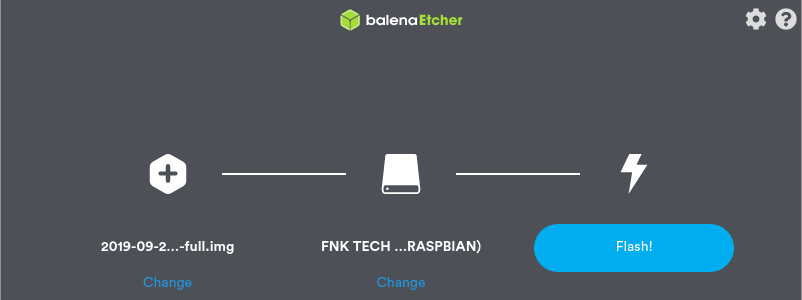
\includegraphics[width=0.9\linewidth,height=8cm,keepaspectratio]{img/p01-02-linux-imageb.png} %CHKTEX 8
		\caption{Listo para grabar la imagen}
		\label{fig:write-image-linux-b} %CHKTEX 24
	\end{subfigure}
	\caption{Escritura de la imagen IMG de Raspbian en la microSD con Etcher}%
	\label{fig:write-image-linux} %CHKTEX 24
\end{figure}

Cuando la escritura de datos en la microSD termine, notará que ésta ha sido reparticionada en \texttt{boot} (partición de arranque tipo \textit{FAT32}) y \texttt{rootfs} (partición raíz tipo \textit{EXT4}).

Si no cuenta con monitor, teclado o mouse, consulte el \Cref{sec:annex1}.
De otro modo, desmonte la tarjeta microSD e insértela en la Raspberry Pi.

% %% %%%%%%%%%%%%%%%%%%%%%%%%%%%%%%%%%%%%%%%%%%%%%%%%%%%%%%%%%%%%%%%%%%
%
% Step 2b: Windows
%
% %% %%%%%%%%%%%%%%%%%%%%%%%%%%%%%%%%%%%%%%%%%%%%%%%%%%%%%%%%%%%%%%%%%%
\subsubsection{Escribir imagen usando Windows}%
Descargue e instale \href{https://sourceforge.net/projects/win32diskimager/}{Win32 Disk Imager}.
Si no ha descmprimido la imagen de Raspbian, proceda a hacerlo con un programa que descomprima archivos Zip como \href{https://www.7-zip.org/download.html}{7zip} (Windows 7 y posterior deberí soportar descompresión zip).

A continuación, siga los pasos de Win32 Disk Imager para grabar la imagen (véase \Cref{fig:write-image-windows})
\begin{enumerate}[noitemsep]
	\item Seleccione la imagen IMG de Raspbian en \emph{Image File}
	\item Seleccione la unidad en la cual se grabará la imagen de Raspbian (letra asignada a la microSD) en \emph{Device}
	\item De click en \emph{Write} para iniciar el proceso de escritura.
	\item Win32 Disk Imager mostrará una advertencia, de click en \emph{Yes} para continuar.
\end{enumerate}

\begin{figure}[H]
	\centering%
	\begin{subfigure}[b]{0.5\linewidth}
		\centering
		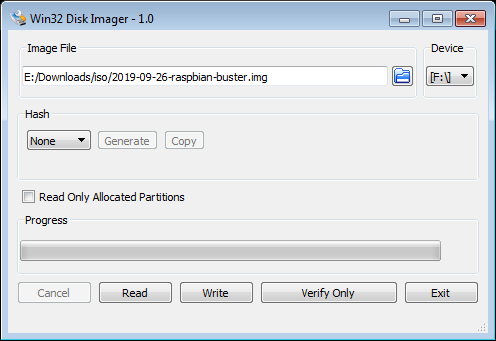
\includegraphics[width=0.9\linewidth,height=8cm,keepaspectratio]{img/p01-02-windows-imagea.png} %CHKTEX 8
		\caption{Selección de imagen a grabar}
		\label{fig:write-image-windows-a} %CHKTEX 24
	\end{subfigure}%
	\begin{subfigure}[b]{0.5\linewidth}
		\centering
		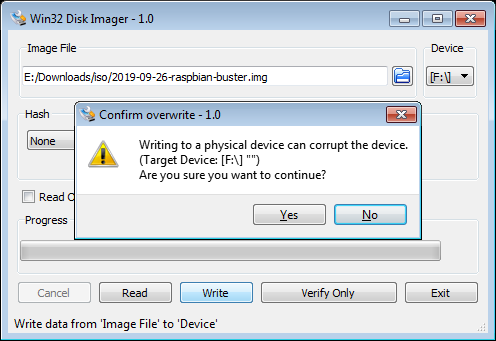
\includegraphics[width=0.9\linewidth,height=8cm,keepaspectratio]{img/p01-02-windows-imageb.png} %CHKTEX 8
		\caption{Listo para grabar la imagen}
		\label{fig:write-image-windows-b} %CHKTEX 24
	\end{subfigure}
	\caption{Escritura de la imagen IMG de Raspbian en la microSD con Win32 Disk Imager}%
	\label{fig:write-image-windows} %CHKTEX 24
\end{figure}

Cuando la escritura de datos en la microSD termine, Windows asignará una letra al nuevo volúmen de datos de la microSD, llamada \texttt{boot}.
Desmonte la tarjeta microSD e insértela en la Raspberry Pi.

% %% %%%%%%%%%%%%%%%%%%%%%%%%%%%%%%%%%%%%%%%%%%%%%%%%%%%%%%%%%%%%%%%%%%
%
% Step 3
%
% %% %%%%%%%%%%%%%%%%%%%%%%%%%%%%%%%%%%%%%%%%%%%%%%%%%%%%%%%%%%%%%%%%%%
\clearpage
\subsection{Paso 3: Configurar Raspbian}%
Para configuar Raspbian, la Raspberry Pi deberá tener una tarjeta de memoria microSD con una imagen de Raspbian precargada y estar conectada a un monitor vía el puerto HDMI incorporado.
Además, se precisa de un teclado y apuntador (mouse) USB para realizar el proceso de configuración.
A continuación, conecte la Raspberry Pi y espere entre 1 y 3 minutos a que el sistema operativo cargue.

\begin{figure}[H]
	\centering
	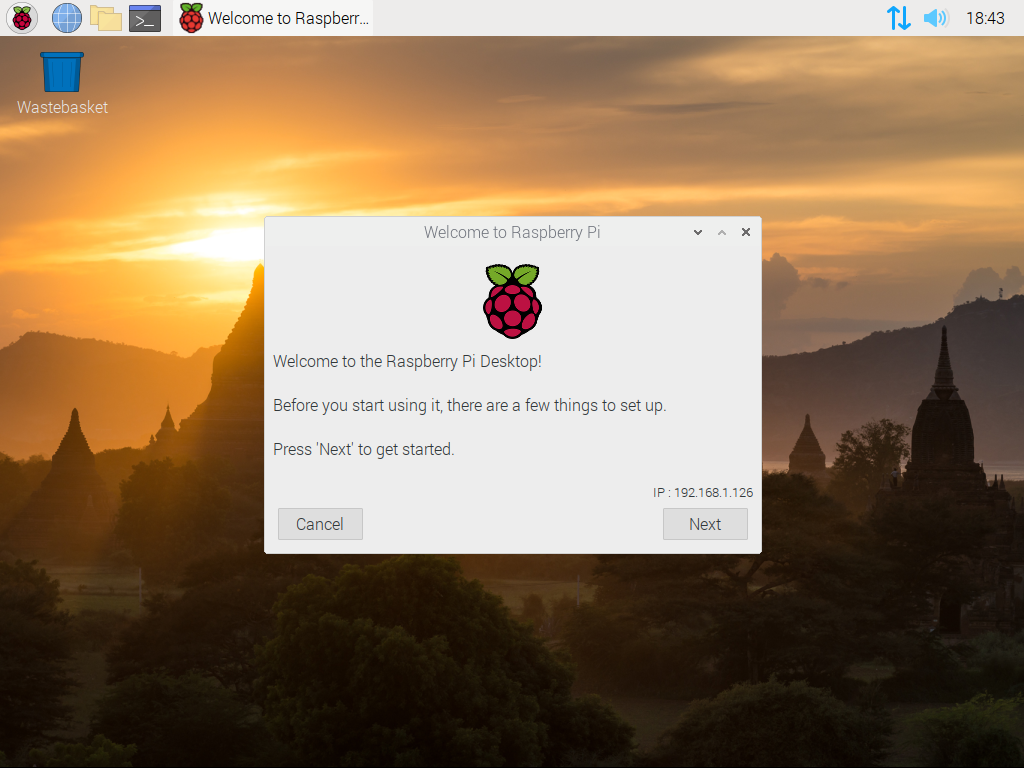
\includegraphics[width=0.9\linewidth,height=8cm,keepaspectratio]{img/p01-03-desktop.png} %CHKTEX 8
	\caption{Escritorio de Raspbian}
	\label{fig:raspbian-desktop} %CHKTEX 24
\end{figure}

Una vez terminado el proceso de arranque, siga el asistente para configurar Raspbian, tal como se muestra en la \Cref{fig:setup-wizard}.


\begin{figure}[H]
	\centering%
	\begin{subfigure}[b]{0.33\linewidth}
		\centering
		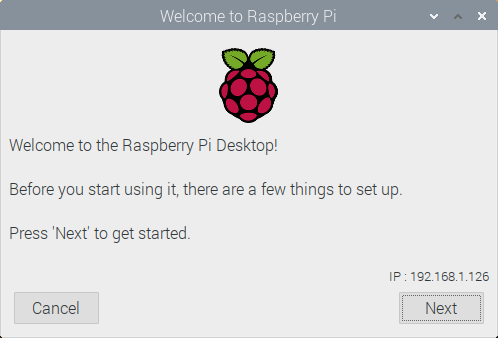
\includegraphics[width=0.9\linewidth,height=33mm,keepaspectratio]{img/p01-03-wizard-1.png} %CHKTEX 8
		\caption{Inicio del\\Asistente de Conficuración\\~}
		\label{fig:setup-wizard-step-1} %CHKTEX 24
	\end{subfigure}%
	\begin{subfigure}[b]{0.33\linewidth}
		\centering
		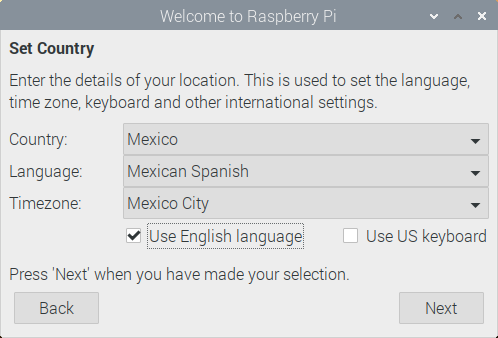
\includegraphics[width=0.9\linewidth,height=33mm,keepaspectratio]{img/p01-03-wizard-2.png} %CHKTEX 8
		\caption{Selección de idioma\\y datos de localización\\~}
		\label{fig:setup-wizard-step-2} %CHKTEX 24
	\end{subfigure}%
	\begin{subfigure}[b]{0.33\linewidth}
		\centering
		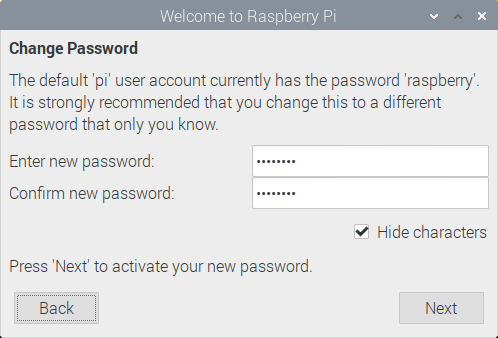
\includegraphics[width=0.9\linewidth,height=33mm,keepaspectratio]{img/p01-03-wizard-3.png} %CHKTEX 8
		\caption{Cambio de contraseña\\del usuario principal \textit{pi}\\~}
		\label{fig:setup-wizard-step-3} %CHKTEX 24
	\end{subfigure}\\
	\begin{subfigure}[b]{0.33\linewidth}
		\centering
		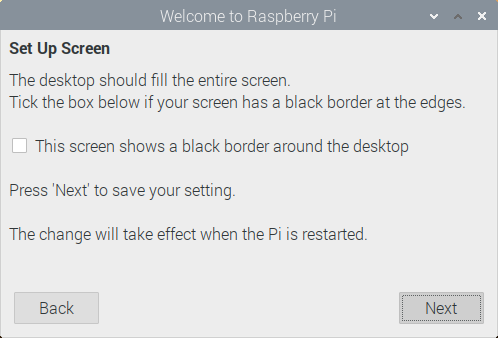
\includegraphics[width=0.9\linewidth,height=33mm,keepaspectratio]{img/p01-03-wizard-4.png} %CHKTEX 8
		\caption{Calibración de pantalla\\~}
		\label{fig:setup-wizard-step-4} %CHKTEX 24
	\end{subfigure}%
	\begin{subfigure}[b]{0.33\linewidth}
		\centering
		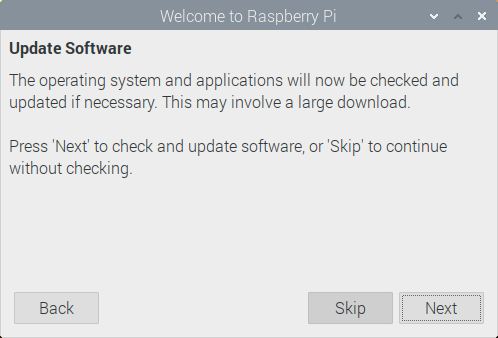
\includegraphics[width=0.9\linewidth,height=33mm,keepaspectratio]{img/p01-03-wizard-5.png} %CHKTEX 8
		\caption{Actualización de Software\\Requiere conexión a internet}
		\label{fig:setup-wizard-step-5} %CHKTEX 24
	\end{subfigure}%
	\begin{subfigure}[b]{0.33\linewidth}
		\centering
		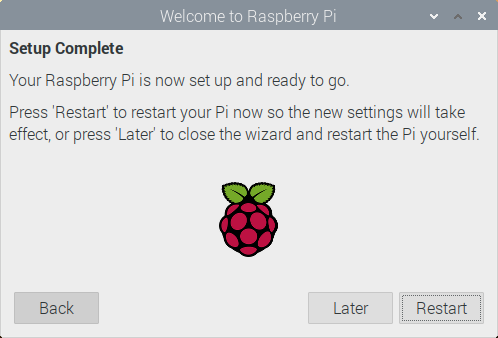
\includegraphics[width=0.9\linewidth,height=33mm,keepaspectratio]{img/p01-03-wizard-6.png} %CHKTEX 8
		\caption{Fin del asistente y reinicio\\~}
		\label{fig:setup-wizard-step-6} %CHKTEX 24
	\end{subfigure}\\
	\caption{Asistente de configuración de Raspbian}%
	\label{fig:setup-wizard} %CHKTEX 24
\end{figure}

Finalmente, se aconseja expandir la partición de Raspbian a su máxima capacidad.
Para ello, ejecute en una terminal la herramienta de configuración \texttt{sudo raspi-config} (véase \Cref{fig:raspberry-config-tool}), seleccione la opción 7, \textit{Opciones avanzadas} (Avanced Options), y luego la opción A1, \textit{Extender el sistema de archivos} (Expand Filesystem).


% %% %%%%%%%%%%%%%%%%%%%%%%%%%%%%%%%%%%%%%%%%%%%%%%%%%%%%%%%%%%%%%%%%%%
%
% Anex
%
% %% %%%%%%%%%%%%%%%%%%%%%%%%%%%%%%%%%%%%%%%%%%%%%%%%%%%%%%%%%%%%%%%%%%
\appendix%
% \clearpage%
\section{Instalación de Raspbian via SSH}%
\label{sec:annex1}
En caso de que no se cuente con un monitor, es posible instalar Raspbian vía SSH. %CHKTEX 13
Para ello es necesario habilitar conexiones vía SSH ya que estas se encuentran deshabilitadas por defecto.


\subsection{Habiliar conexiones SSH}
\label{sec:annex1-ssh-enable}
Para habilitar SSH, se necesita crear un archivo vacío llamado \texttt{SSH} en la raíz de la partición \texttt{rootfs}.
Supóngase que la microSD está asociada a \texttt{/dev/sdc}, las paticiones \texttt{boot} y \texttt{rootfs} serán entonces \texttt{/dev/sdc1} y \texttt{/dev/sdc2} respectivamente.
El proceso de creación del archivo \texttt{SSH} en la raíz de la partición \texttt{rootfs} es como sigue:

\begin{Verbatim}[fontsize=\footnotesize]
$ mkdir /media/user/rootfs
# mount /dev/sdc2 /media/user/rootfs
# touch /media/user/rootfs/SSH
\end{Verbatim}

Nótese que los comandos marcados con \texttt{\#} deben ejecutarse con permisos de super usuario (i.e.~\emph{root}, o mediante \texttt{sudo} en Ubuntu).

Una vez completado este proceso, desmonte la memoria microSD e insértela en la Raspberry Pi.

\subsection{Configurar Raspbian vía SSH}
Para configuar Raspbian via SSH, la Raspberry Pi deberá estar conectada a la red local vía un cable Ethernet y tener una tarjeta de memoria microSD con una imagen de Raspbian precargada.

A continuación, conecte la Raspberry Pi y espere entre 1 y 3 minutos a que el sistema operativo cargue.
Utilice un escaner de IP o consulte su enrutador para conocer la IP asignada a la Raspberry Pi.

\begin{figure}[H]
	\centering%
	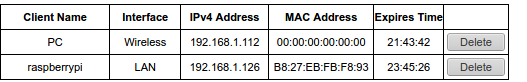
\includegraphics[width=9cm]{img/p01-appendix01.png} %CHKTEX 8
	\caption{Dirección IP de una Raspbery Pi}
	\label{fig:raspberry-ip} %CHKTEX 24
\end{figure}

Una vez conozca la dirección IP de la Raspberry Pi, conéctese a ésta mediante SSH. %CHKTEX 13
Secure Shell le advertirá que no puede verificar la autenticidad del certificado, por lo que pedirá que confirme la conexión tecleando \texttt{yes}, como se muestra a continuación.

\begin{Verbatim}[fontsize=\footnotesize]
$ ssh pi@192.168.1.126

    The authenticity of host '192.168.1.126 (192.168.1.126)' can't be established.
    ECDSA key fingerprint is SHA256:1nrpQeTIb+Gzg4aIJ0WE+V0aLUQgDnQbxOGraWf0Kso.
    Are you sure you want to continue connecting (yes/no)?
\end{Verbatim}

Teclee \texttt{yes} y presione Enter.
De inmediato se le solicitará la contraseña

\begin{Verbatim}[fontsize=\footnotesize]
    Warning: Permanently added '192.168.1.126' (ECDSA) to the list of known hosts.

    pi@192.168.1.126's password:
\end{Verbatim}

Teclee \texttt{raspberry}, la contraseña por default en Raspbian, y presione Enter.
Se concretará la conexión.

\begin{Verbatim}[fontsize=\footnotesize]
    Linux raspberrypi 4.19.75-v7+ #1270 SMP Tue Sep 24 18:45:11 BST 2019 armv7l

    The programs included with the Debian GNU/Linux system are free software;
    the exact distribution terms for each program are described in the
    individual files in /usr/share/doc/*/copyright.

    Debian GNU/Linux comes with ABSOLUTELY NO WARRANTY, to the extent
    permitted by applicable law.
    Last login: Thu Feb  6 18:28:53 2020

    SSH is enabled and the default password for the 'pi' user has not been changed.
    This is a security risk - please login as the 'pi' user and type 'passwd' to set a new password.
\end{Verbatim}

Finalmente, para configurar su Raspbian, ejecute \texttt{sudo raspi-config}  para iniciar la herramienta de configuración (véase \Cref{fig:raspberry-config-tool}).
Se aconseja definir el idioma, localización, y cambiar la contraseña del usuario por defecto \textit{pi}.

\begin{figure}[H]
	\centering%
	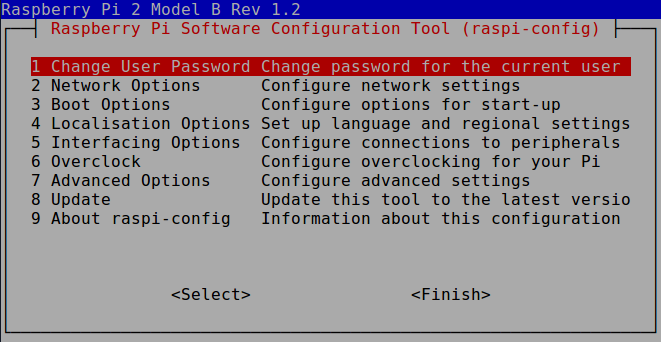
\includegraphics[width=0.8\linewidth,height=5cm,keepaspectratio]{img/p01-appendix02.png} %CHKTEX 8
	\caption{Herramienta de configuración de Raspbian}
	\label{fig:raspberry-config-tool} %CHKTEX 24
\end{figure}

\end{document}
